\documentclass[11pt]{beamer}

 \usepackage{beamerthemesplit} % // Activate for custom
\usepackage{amssymb}
\usepackage{amsmath}
\usepackage{enumitem}
\usepackage{graphicx}

%\newcounter{sauvegardeenumi}
%\newcommand{\asuivre}{\setcounter{sauvegardeenumi}{\theenumi}}
%\newcommand{\suite}{\setcounter{enumi}{\thesauvegardeenumi}}

%% or use the epsfig package if you prefer to use the old commands
\usepackage{epsfig}

%% The amssymb package provides various useful mathematical symbols
\usepackage{amssymb}
%% The amsthm package provides extended theorem environments
 \usepackage{amsthm}

%\usepackage{natbib}
%\usepackage{ifsym}
\usepackage[geometry]{ifsym}


\usetheme{Warsaw}
%\setbeamerfont{size*=24pt}
\usecolortheme{rose}
%\setbeamertemplate{itemize subitem}[triangle]
\setbeamertemplate{itemize items}[default]

%\usecolortheme{seahorse}
%Begin Title

\newcommand{\indentitem}{\setlength\itemindent{25pt} \item}
\newcommand{\tenindent}{\setlength\itemindent{10pt} \item[]}
\newcommand{\iitem}{\setlength\itemindent{25pt} \item}
\newcommand{\fiftyindent}{\setlength\itemindent{50pt} \item[]}
\newcommand{\bigindent}{\setlength\itemindent{75pt} \item[]}
\newcommand{\zeroindent}{\setlength\itemindent{0pt} \item}
\newcommand{\backindent}{\setlength\itemindent{-25pt} \item}
\newcommand{\restoreindent}{\setlength\itemindent{0pt} \item}

\newcommand{\myitemb}{\item[(b)]}
\newcommand{\myitemc}{\item[(c)]}
\newcommand{\myitemd}{\item[(d)]}
\newcommand{\myiteme}{\item[(e)]}
\newcommand{\myitemf}{\item[(f)]}

\setbeamerfont{title}{size=\normalsize}

\title[Intro to Variational Inference] %{\fontsize{6pt}} %{size = \tiny}
{An Introduction to Variational Inference}
%{Effects of Population Density on Parameter Estimation in Individual-Level Models of Infectious Disease}
\author[Carolyn Augusta]
{Carolyn Augusta}
\institute[University of Guelph]
{
Department of Mathematics and Statistics\\
University of Guelph\\
}
\date{\small May 19th 2015}
%End Title

\begin{document}
\def\newblock{\hskip .11em plus .33em minus .07em}

\frame{\titlepage}

\setcounter{tocdepth}{1}
%\frame{\tableofcontents}
\AtBeginSection[]
{
  \begin{frame}<beamer>
    \tableofcontents[currentsection]
  \end{frame}
}

\section{Bayesian statistics in a nutshell}

\frame
{
\frametitle{General philosophy}
	\begin{itemize}
		\item Frequentist statisticians don't assign a probability to an event before they perform an experiment
		\indentitem E.g. if they'd never seen a die before, a frequentist would roll it over and over and after some large number of rolls, would say the probability of seeing a '1' is roughly 1/6
		\zeroindent Bayesian statisticians assign a probability to an event, then perform an experiment
		\indentitem E.g. look at the die before you roll it, see it has 6 faces, guess the probability of '1' is roughly 1/6. Then start rolling.
	\end{itemize}

}

\frame
{
\frametitle{Why Bayesian statistics?}
	\begin{itemize}
		\item Frequentist statisticians look at long-range frequencies of events to derive probabilities
		\indentitem E.g. roll that die 24,000 times and count the number of '1's you see.
		\item Bayesian statisticians can give you a rough idea of the probability of an event before they see any results
		\indentitem E.g. The probability that it will rain this afternoon
		\item Notice the weather is not a repeatable event - you can't see the weather this afternoon more than once. So the frequentist paradigm doesn't really make sense to use here. You can't see this afternoon's weather 24,000 times and count how many times it rained.
		\item Note - that's a controversial statement. It's just an example to get you thinking along these lines.
		\item Also note that's just one use of Bayesian statistics, but it's the one I find most intuitive.
	\end{itemize}
}

\frame
{
\frametitle{Bayesian inference}
	\begin{itemize}
	\item Often when we conduct an experiment, we're interested in finding a model describes the data
	\item Suppose we expect a simple linear regression model will be a good fit to our data: ${\hat{y}} = \hat{\beta_0} + \hat{\beta_1}x$. We want the line of best fit (find $\beta_0$ and $\beta_1$)
	\item Let $\theta = (\beta_0, \beta_1)$
	\end{itemize}
}


\begin{frame}[t]
\begin{columns}[T] % align columns
\begin{column}{.60\textwidth}
%\color{red}\rule{\linewidth}{4pt}
 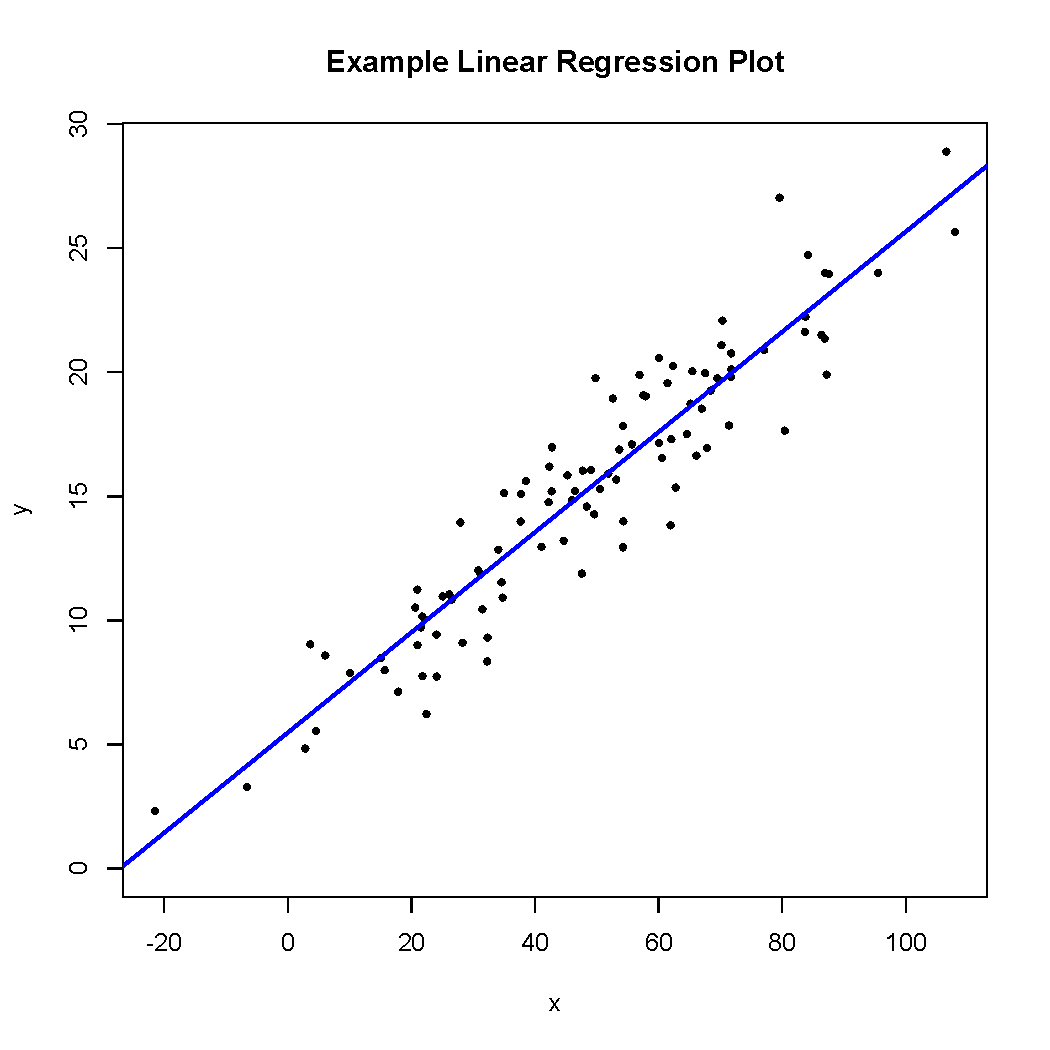
\includegraphics[scale=0.4]{ExampleLinReg.pdf} 
 {\vspace{-0.1in}}

 \begin{equation*}
 \hat{y} = \hat{\beta_0} + \hat{\beta_1} x
 \end{equation*}

%Left Part
\end{column}%
\hfill%
\begin{column}{.40\textwidth}
%\color{blue}\rule{\linewidth}{4pt}

%Right Part
 We want to find the best values of $\theta$, given what we see in our data. So we want to infer $\theta$ from the conditional distribution of $\theta$ given our data. This is called the {\textbf{posterior distribution}}, and is denoted $\mathbf{P(\theta \mid y)}$

\end{column}%
\end{columns}
\end{frame}

%%%%%

\begin{frame}[t]
\begin{columns}[T] % align columns
\begin{column}{.60\textwidth}
%\color{red}\rule{\linewidth}{4pt}
 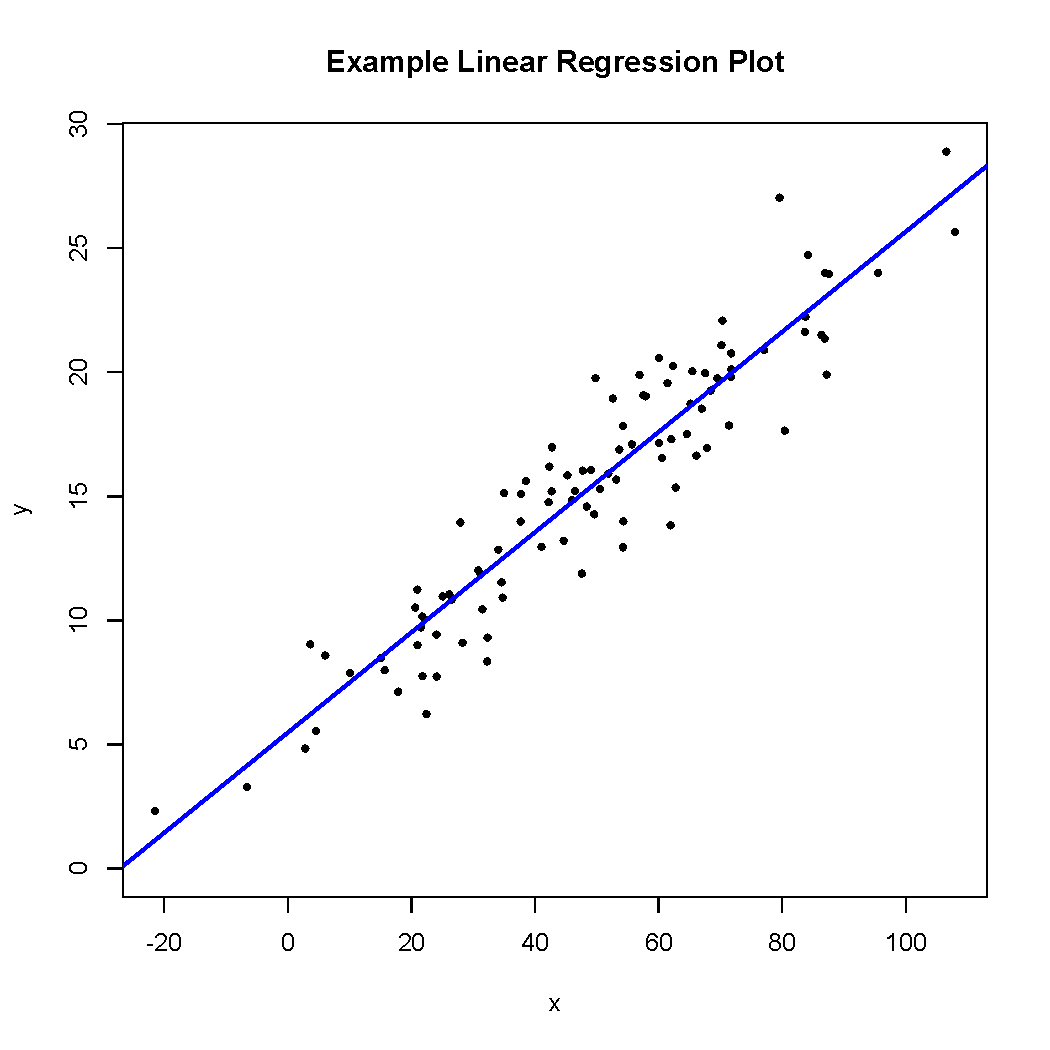
\includegraphics[scale=0.4]{ExampleLinReg.pdf} 
 {\vspace{-0.1in}}

 \begin{equation*}
 \hat{y} = \hat{\beta_0} + \hat{\beta_1} x
 \end{equation*}

%Left Part
\end{column}%
\hfill%
\begin{column}{.40\textwidth}
%\color{blue}\rule{\linewidth}{4pt}

%Right Part
 {\textbf{posterior}}: $\mathbf{P(\theta \mid y)}$ \\
 
 \vspace{0.25in}
Since we're working in a Bayesian framework, we have some guess of what $\beta_0$ and $\beta_1$ should be, before we even see the data $y$ (maybe from previous work). So we have rough initial guess of the values of $\beta_0$ and $\beta_1$, and how they vary. This is called the $\textbf{prior distribution}$ of $\theta$, and is denoted $\mathbf{P(\theta)}$

\end{column}%
\end{columns}
\end{frame}

%%%%%

\frame[t]
{
\begin{columns}[T] % align columns
\begin{column}{.60\textwidth}
%\color{red}\rule{\linewidth}{4pt}
 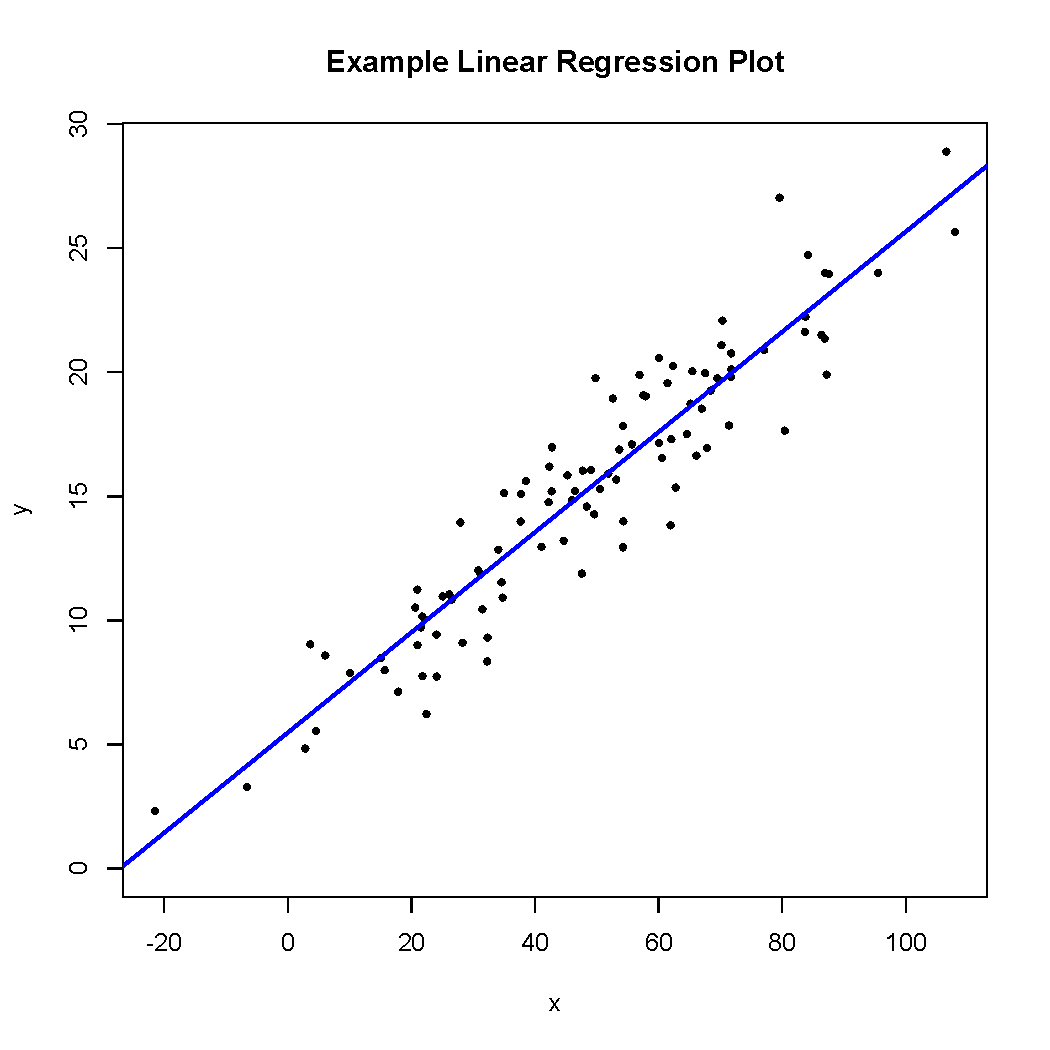
\includegraphics[scale=0.4]{ExampleLinReg.pdf} 
 {\vspace{-0.1in}}

 \begin{equation*}
 \hat{y} = \hat{\beta_0} + \hat{\beta_1} x
 \end{equation*}

%Left Part
\end{column}%
\hfill%
\begin{column}{.40\textwidth}
%\color{blue}\rule{\linewidth}{4pt}

%Right Part
 {\textbf{posterior}}: $\mathbf{P(\theta \mid y)}$ \\
 {\textbf{prior}}: $\mathbf{P(\theta)}$ \\
 
 \vspace{0.1in}

We have data $y$, and we have some ``best guess so far" values $\theta$. We can look at the probability that the data we see was generated by a model with our ``best guess" parameter values. This is called the {\textbf{likelihood}}, and is denoted $\mathbf{P(y \mid \theta)}$ \\
 \vspace{0.1in}
Now we need a relationship among all these distributions.

\end{column}%
\end{columns}
}


\frame[t]
{
\frametitle{Bayes' Theorem from Conditional Probability}

\begin{columns}[T] % align columns
\begin{column}{.60\textwidth}
%\color{red}\rule{\linewidth}{4pt}
	\begin{equation}
	P(\theta \mid y) = \frac{P(y, \theta)}{P(y)}
	\end{equation}
	\vspace{0.1in}
	\begin{equation}
	P(y \mid \theta) = \frac{P(y, \theta)}{P(\theta)}
	\end{equation}
	\vspace{0.1in}	
	\begin{equation}
	P(y, \theta) = P(y \mid \theta) P(\theta)
	\end{equation}
	\vspace{0.1in}	
	\begin{equation}
	P(\theta \mid y) = \frac{ P(y \mid \theta) P(\theta)}{P(y)}
	\end{equation}	


\end{column}%
\hfill%
\begin{column}{.40\textwidth}
	\vspace{0.1in}
by definition of conditional probability \\
\vspace{0.25in}
also by definition of conditional probability \\
\vspace{0.2in}
rearranging (2) \\
\vspace{0.3in}
plugging (3) into (1) - Bayes' Theorem! \\

\end{column}%
\end{columns}

%	Recall from conditional probability: 
%
%	
%	But we can also say:
%	
%	\begin{equation}
%	P(y \mid \theta) = \frac{P(y, \theta)}{P(\theta)}
%	\end{equation}
%	
%	So, rearranging (2):
%	
%	\begin{equation}
%	P(y, \theta) = P(y \mid \theta) P(\theta)
%	\end{equation}
%	
%	and substituting (3) into (1):
%	
%	\begin{equation}
%	P(\theta \mid y) = \frac{ P(y \mid \theta) P(\theta)}{P(y)}
%	\end{equation}	
			
	
	

%	\begin{equation*}
%	P(\theta \mid y) = \displaystyle{\frac{P(y \mid \theta) P(\theta)}{P(y)}}
%	\end{equation*}
%	where \\
%	\vspace{0.1in}	
%	$P(\theta \mid y)$ is the {\textbf{posterior distribution}} - the probability of the model parameters $\theta$ given the data that we see, $y$ \\
%	\vspace{0.1in}	
%	$P(y \mid \theta)$ is the \textbf{likelihood} -  the probability of seeing the data, given the model parameters that we chose \\
%	\vspace{0.1in}	
%	$P(\theta)$ is the {\textbf{prior distribution}} - the probability of the model parameters taking certain values, before we see any data \\
	%\vspace{0.1in}	
	%$P(y)$ is the {\textbf{normalizing constant}} - the probability of the data alone, regardless of the model parameters.
	
}

\frame[t]
{
\frametitle{So what's the problem?}

	\begin{equation*}
	P(\theta \mid y) = \displaystyle{\frac{P(y \mid \theta) P(\theta)}{P(y)}}
	\end{equation*}

Look again at the normalizing constant, $P(y)$ \\
	\vspace{0.1in}	
To get that value, we'd have to marginalize over all values $\theta$ could take:
$P(y) = \int_{\theta} P(y \mid \theta) P(\theta) d\theta$ \\
	\vspace{0.1in}	
	
In a lot of cases, the number of parameters in our model is large, so we'd have to integrate over a huge space. 
 The normalizing constant becomes computationally intractable, which makes the posterior intractable. \\
	\vspace{0.1in}	
We need {\textbf{approximate inference}} methods to make conclusions about the parameters $\theta$, based on the data $y$. \\
}

\frame
{
	\frametitle{Approximate inference intro}

There are two main frameworks for approximate Bayesian inference: Markov chain Monte Carlo (MCMC) and variational Bayes (VB) methods. \\

Today we'll go over VB with an example using Bayesian linear regression, so you can see how the mechanics work. \\

Then a more complicated example, when inference really is intractable.
}

\section{Bayesian linear regression}

\frame
{
\frametitle{Making Simple Linear Regression Bayesian}
	All we have to do is specify prior distributions over the model parameters.
	Frequentist methods: maximum likelihood and least squares give best values of $\beta_0$ and $\beta_1$
	Bayesian methods: 
}

%\frame
%{
%	\frametitle{How do we make simple linear regression Bayesian?}
%	
%	\begin{itemize}
%		\item Assume we have continuous data $y$ and a single linear predictor $x$, like before
%		\item E.g. Say our experiment had $x$ as temperature. A phenomenon that depends on temperature likely also depends on humidity, but we haven't put that in the model.
%		\item So our data $y$ will vary by some amount $\epsilon$, even if we hold $x$ constant.
%		\begin{equation}
%		Y_i = \beta_0 + \beta_1 x_i + \epsilon_i
%		\end{equation}
%		where $\epsilon_i  \stackrel{iid}{\sim} N(0, \sigma^2)$
%	\end{itemize}
%}
%
%\frame[t]
%{
%	\frametitle{How do we make simple linear regression Bayesian?}
%		
%		\begin{equation*}
%		Y_i = \beta_0 + \beta_1 x_i + \epsilon_i \hspace{0.5in} \epsilon_i \stackrel{iid}{\sim} N(0, \sigma^2)
%		\end{equation*}
%		
%		Is the same as saying
%		
%		\begin{equation*}
%		Y_i \mid x_i = \beta_0 + \beta_1 x_i + \epsilon_i \hspace{0.5in} \epsilon_i \stackrel{iid}{\sim} N(0, \sigma^2)
%		\end{equation*}	
%		
%		\begin{align*}
%		E(Y_i \mid x_i) &= E(\beta_0 +\ \beta_1 x_i + \epsilon_i)
%		&= E(\beta_0) + E(\beta_1x_i) + E(\epsilon_i)
%		&= \beta_0 + \beta_1x_i
%		\end{align*}
%		
%		\begin{align*}
%		Var(Y_i \mid x_i) &= Var(\beta_0 + \beta_1x_i + \epsilon_i)
%		&= Var(\epsilon_i)
%		&= \sigma^2
%		\end{align*}	
%
%		\begin{equation*}
%		P(Y_i \mid x_i) = N(\beta_0 + \beta_1 x_i , \sigma^2)
%		\end{equation*}				
%
%}


\frame
{
\frametitle{Outline}
	\begin{itemize}{\itemsep=0.25in}
		%\item Bayesian statistics in a nutshell
		\item Bayesian philosophy
		\item Bayes' Theorem
		\item The posterior distribution
		\item The normalizing constant
		\item The marginal likelihood
		\item The general idea
		\item The algorithm
		\item Where the algorithm came from
		\item Bayesian mixture models
		\item A step-by-step example using Bayesian mixture models
	\end{itemize}
}



\frame
{
\frametitle{SIR Compartmental Model}
	\begin{itemize}
		\backindent Disease transmission and recovery can be described via a pure-birth process called an SIR model.	
		\vspace{0.05in}	
		\item Suppose all individuals are susceptible to the disease (they are in state ``S")
		\vspace{0.05in}
		\item They become infectious according to a certain probability (move to state ``I")
		\vspace{0.05in}
		\item After $\gamma$ time periods, they are removed from the population due to recovery, acquired immunity, etc. (state ``R")

	\end{itemize}
}

%\frame[t]
%{
%\frametitle{Individual-Level Models}
%
%	\begin{itemize}
%		\backindent One way to model an epidemic is by means of a discrete-time Poisson process (infection events happen in [t, t+1))
%		\vspace{0.05in}
%		\backindent Say Z $\sim Poi(\omega_{it})$
%		\vspace{0.05in}
%		\backindent  Z = number of infection events in [t, t+1)
%		\backindent $\omega_{it}$ = the rate of infection for indiv. i in [t, t+1)
%		\vspace{0.05in}
%    		\backindent $P(Z = z) = {\frac{\displaystyle{exp(-\omega_{it}) w_{it}^z}}{\displaystyle{z!}}}$
%		\vspace{0.1in}
%		\backindent  $P(Z > 0) = 1 - P(Z = 0) = 1 - exp(-\omega_{it})$
%	\end{itemize}
%}

\frame[t]
{
\frametitle{Individual-Level Models}
	
	\begin{itemize}
		\backindent P(infection in [t, t+1)) = $1 - exp(-\omega_{it})$
		\vspace{0.05in}
		\restoreindent  $\omega_{it} = \alpha \sum_{j \in I(t)} {\rm{d_{ij}}}^{-\beta}$,  {\small{$j \in I(t)$ if $t - \gamma \le {\rm{inf(j)}} < t$}}
		%\restoreindent $\omega_{it} = \alpha \sum_{j \in I(t)} {\rm{d_{ij}}}^{-\beta}$ 
		%\restoreindent {\small{$j \in I(t)$ if $t - \gamma \le {\rm{inf(j)}} < t$}}
		\vspace{0.05in}
		\item $\alpha$: susceptibility, set prior: $\alpha \sim U(0, 50)$
		\vspace{0.05in}
		\item $I(t)$: set of infectious individuals at time t
		\vspace{0.05in}
		\item $d_{ij}$: (Euclidean) distance between susceptible $i$ and infectious $j$
		\vspace{0.05in}
		\item $\beta$: spatial effect, set prior: $\beta \sim U(-5, 50)$
		\vspace{0.05in}
		\item $\gamma$: infectious period, set prior: $\gamma \sim DU[1,10]$
	\end{itemize}

}

%\frame[t]
%{
% \frametitle{First population, MVN([i,i], [1,1,1,1]) }
%	\vspace{-0.4cm}
%	Epidemic with $\alpha = \beta = \gamma = 1.0$
%	\begin{center}
%	\vspace{-0.4cm}
%	\includegraphics[scale=0.45]{PopulationPlot-111-1.pdf}
%	\end{center}
%}
%
%\frame[t]
%{
% \frametitle{First population, MVN([i,i], [1,1,1,1]) }
%
%	\begin{center}
%	\vspace{-0.5cm}
%	\includegraphics[scale=0.45]{MCMCTraceAlphaPop1-111-1.pdf}
%	\end{center}
%}

\frame[t]
{
 \frametitle{References}

Deardon, R. et al. (2010). Inference for individual-level models of infectious diseases in large populations. Statistica Sinica, 20, 239-261. \\
\vspace{0.25in}
Gold, J. (2015). Computational inference for network-based individual-level models of infectious disease transmission (Unpublished doctoral dissertation). University of Guelph, Guelph Ontario Canada.
}

\end{document}
